\section{Verificadores de modelos}

La elección de un verificador de modelos adecuado es una parte vital de este trabajo porque es
el responsable de verificar la ausencia de bloqueos. Afortunadamente se han desarrollado
varios comprobadores de modelos para analizar redes de Petri.

El \acrfull{MCC} \cite{khhjp2021} organizado en la
Universidad de la Sorbona de París es una gran fuente de verificadores de modelos de última
generación. Se trata de un concurso anual en el que los verificadores de modelos presentados
se ejecutan sobre una serie de modelos de redes de Petri procedentes del mundo académico y de la
industria\footnote{\url{https://mcc.lip6.fr/2023/models.php}}.
Estos modelos han sido aportados por muchas personas a lo largo de un periodo de
más de una década y el número total de puntos de referencia ha crecido paulatinamente a
medida que se han ido añadiendo nuevos modelos.

Cada año, los puntos de referencia incluyen redes de lugares/transiciones (\acrfull{P/T nets}), es
decir, redes de Petri, y redes de Petri coloreadas (\acrfull{CPN}). El número de lugares en las redes
puede oscilar entre una docena y más de 70000 y las transiciones entre menos de un
centenar y más de un millón. Esto pone de manifiesto la aplicabilidad práctica de los
verificadores de modelos que participan en el concurso.

Los resultados se publican en la página web oficial (véase por ejemplo \cite{mcc:2022}) y
consisten en:

\begin{enumerate}
      \item una lista de las herramientas cualificadas que participaron,
      \item las técnicas aplicadas en cada una de las herramientas,
      \item una sección dedicada a detallar las condiciones experimentales en las que se desarrolló el
            concurso (el hardware utilizado y el tiempo necesario para completar las ejecuciones),
      \item los resultados en forma de tablas, gráficos e incluso los registros de ejecución de cada programa,
      \item la lista de ganadores de cada categoría,
      \item un análisis de la fiabilidad de las herramientas basado en la comparación de los resultados.
\end{enumerate}

Un breve vistazo a las diapositivas de la edición de 2022\footnote{\url{https://mcc.lip6.fr/2022/pdf/MCC-PN2022.pdf}}
reproducidas en la Fig. \ref{fig:mcc2022-tools} ilustra que varios verificadores de modelos han demostrado una participación ininterrumpida, con ejemplos
notables que incluyen:

\begin{itemize}
      \item \acrfull{TAPAAL} mantenida
            por la Universidad de Aalborg en Dinamarca\footnote{\url{https://www.tapaal.net/}},
            ganadora de una medalla de oro en la edición de 2023.
      \item \acrfull{LoLA} mantenido por la Universidad de
            Rostock en Alemania\footnote{\url{https://theo.informatik.uni-rostock.de/theo-forschung/tools/lola/}},
            ganador en ediciones anteriores y fue utilizado base para otros verificadores de modelos.
      \item ITS-tools \cite{thierrymieg:hal-02104373},
            que también se combinó con \acrshort{LoLA} y obtuvo medallas en
            2020\footnote{\url{https://github.com/yanntm/its-lola}}.
\end{itemize}

\begin{figure}[!htb]
      \centering
      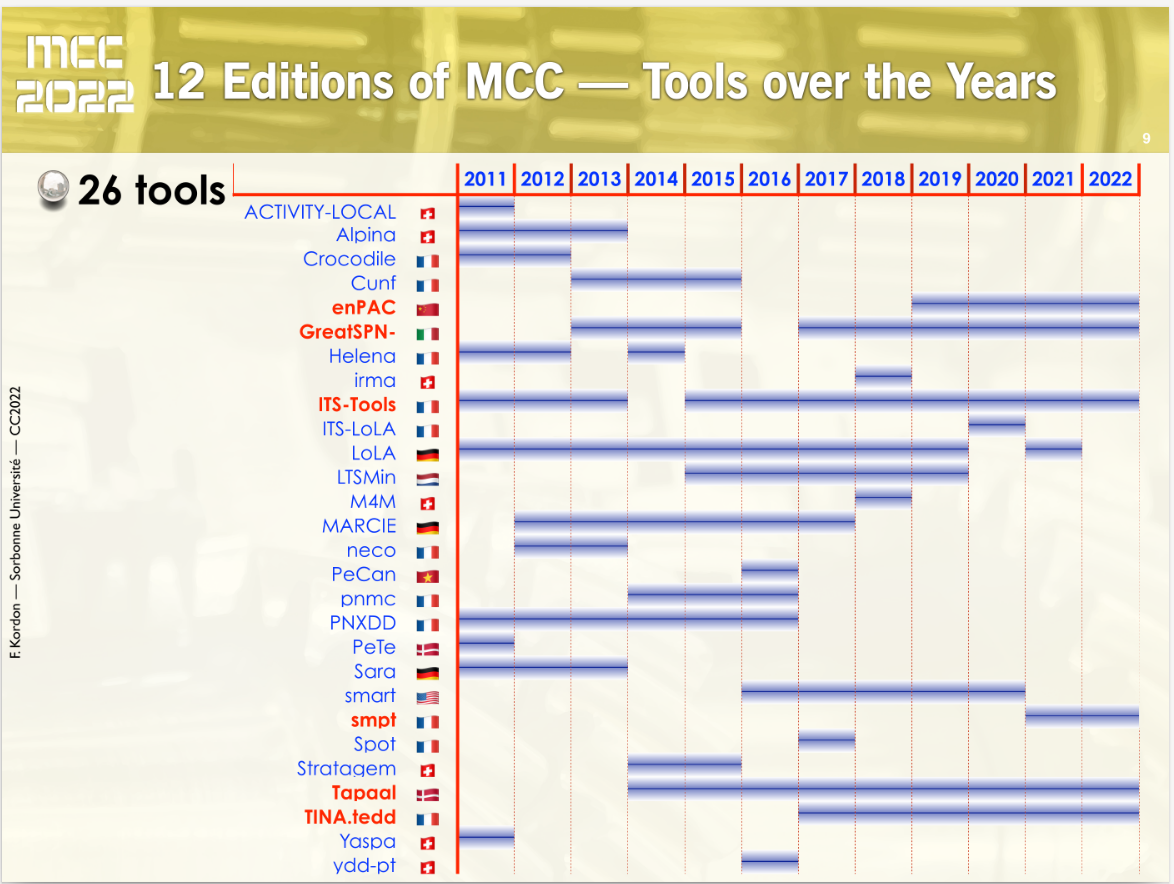
\includegraphics[width=\linewidth]{mcc2022-tools.png}
      \caption{Participación de los verificadores de modelos en el MCC a lo largo de los años.}
      \label{fig:mcc2022-tools}
\end{figure}

Estas observaciones indican colectivamente la madurez y vitalidad de la comunidad de
verificadores de modelos. El establecimiento de un panorama de herramientas bien
desarrollado, fomentado por la colaboración y la difusión de código abierto de resultados, \textit{benchmarks} y técnicas,
presenta una valiosa oportunidad para aprovechar estas herramientas en el ámbito del
desarrollo de software. Concretamente, en el contexto de integrarlas como backends para un
traductor para un lenguaje de programación específico que se encargue de automatizar el proceso de creación de
modelos de redes de Petri. Capitalizando los esfuerzos académicos invertidos en los
verificadores de modelos, se puede lograr una mayor seguridad y fiabilidad en los proyectos
de software.
